\documentclass{BeamerTemplate}
\title{Module 6 - Statistiques descriptives}
\subtitle{STT-1000 Probabilités et statistique}
\date{\today}

% Lien discret vers la page de réponses, ajouté au pied de page à côté du numéro
% (ne prend aucune place sur la diapo). Usage, n'importe où dans la diapo : \lienreponse{rep-ex}
\newcommand{\cibleReponse}{}
\newcommand{\lienreponse}[1]{\gdef\cibleReponse{#1}}
\addtobeamertemplate{footline}{}{%
  \ifx\cibleReponse\empty\else
    \begin{tikzpicture}[remember picture,overlay]
      \node[anchor=south east, inner sep=0pt] at ([xshift=-1.5cm,yshift=0.2cm]current page.south east)
        {\hyperlink{\cibleReponse}{\scriptsize\color{gray}Réponse~$\rightarrow$}};
    \end{tikzpicture}%
    \global\let\cibleReponse\empty
  \fi}
% Lien de retour vers l'exemple, dans les pages de réponses
\newcommand{\retour}[2]{\hyperlink{#1}{\textbf{#2}~{\color{gray}$\hookleftarrow$}}}

% Graphiques (données exactes des anciennes images). Les styles sont définis ici,
% avant \begin{document} : babel-french rend « : » actif ensuite (domain=a:b).
\pgfplotsset{
  % diagramme de points : une observation par point, empilées si égales
  diagpoints/.style={
    scale only axis, width=4.6cm, y=0.17cm, ymin=0.3,
    axis x line=bottom, axis y line=none,
    tick label style={font=\scriptsize}, xtick align=outside,
  },
  pts/.style={only marks, mark=*, mark size=1.7pt, color=black!65},
  % histogrammes de l'exemple 4
  histo/.style={
    width=5.9cm, height=4.6cm, axis lines=left, ymin=0,
    tick label style={font=\tiny}, label style={font=\scriptsize},
    xlabel={Utilisation du processeur (\%)},
    ymajorgrids, grid style={gray!25}, axis on top=false,
    scaled y ticks=false,
    yticklabel style={/pgf/number format/.cd, fixed, fixed zerofill, precision=2, use comma},
    xticklabel style={/pgf/number format/.cd, use comma},
  },
  % densités du quiz sur la moyenne et la médiane théoriques
  quizloi/.style={
    width=6.2cm, height=2.9cm, axis lines=left, ymin=0,
    tick label style={font=\tiny}, scaled y ticks=false,
    yticklabel style={/pgf/number format/.cd, fixed, use comma},
    xticklabel style={/pgf/number format/.cd, use comma},
  },
  dom-beta/.style={domain=0:0.83, samples=120},
}

\begin{document}

\begin{frame}
\titlepage
\end{frame}

% ============================================================================
\section{Introduction}

\begin{frame}[t]{Jeu de données statistique}

Un jeu de données est habituellement constitué de \alerter{plusieurs observations} de
\alerter{plusieurs variables}.

\medskip
{\small
Exemple de mesures recueillies lors d'exécutions successives d'un programme :

{\scriptsize
\begin{center}
\begin{tabular}{ccccc}\hline
Exécution & Temps (s) & Cache activé & Niveau d'optimisation & Température de la salle ($^\circ$C) \\ \hline
1 & 12,0 & Oui & Bas & 17 \\
2 & 13,5 & Non & Moyen & 15 \\
3 & 11,5 & Non & Élevé & 14 \\
4 & 13,0 & Oui & Moyen & 18 \\
5 & 14,0 & Non & Bas & 21 \\
$\vdots$&$\vdots$&$\vdots$&$\vdots$&$\vdots$\\\hline
\end{tabular}
\end{center}
}

\begin{itemize}
\item Variables qualitatives ou quantitatives (traitées différemment en statistique).
\item Nous étudierons les variables \alerter{quantitatives} dans ce cours.
\end{itemize}
}
\end{frame}


\begin{frame}[t]{Décrire avant d'analyser}
Une bonne analyse commence par un \alerter{résumé} de la distribution des observations.

\uncover<2->{
\begin{enumerate}[$\bullet$]\itemsep0pt
\item mesures de \alerter{position}
    {\small\begin{enumerate}[$\circ$]\itemsep0pt
    \item {\color{gray}{moyenne}}
    \item {\color{gray}{médiane}}
    \item {\color{gray}{autres quantiles}}
    \item {\color{gray}{mode}}
    \end{enumerate}}
\item mesures de \alerter{dispersion}
    {\small\begin{enumerate}[$\circ$]\itemsep0pt
    \item {\color{gray}{variance et écart-type}}
    \item {\color{gray}{écart interquartile}}
    \item {\color{gray}{étendue}}
    \end{enumerate}}
\item représentations \alerter{graphiques}
    {\small\begin{enumerate}[$\circ$]\itemsep0pt
    \item {\color{gray}{histogramme}}
    \item {\color{gray}{diagramme en boîte}}
    \item {\color{gray}{diagramme quantile-quantile (au module 10)}}
    \end{enumerate}}
\end{enumerate}
}
\end{frame}


\begin{frame}[t]{Types de variables}
\vspace{-0.4cm}
{\footnotesize
Les variables observées sont généralement de l'un de trois types :
\begin{itemize}\itemsep0pt
\item<1-> \textbf{Variable quantitative :} variable dont la valeur est un nombre entier ou un nombre réel
(p.\,ex. un temps d'exécution, une température, un nombre de bogues).
\item<2-> \textbf{Variable qualitative :}
 \begin{itemize}\itemsep0pt
  \item<2-> \textbf{Variable qualitative ordinale :} variable dont la valeur n'est \alert{pas une mesure
  continue ou un dénombrement}, mais dont les modalités peuvent être \alert{ordonnées}
  (p.\,ex. la priorité d'un billet de soutien : « basse », « moyenne », « haute »).
  \item<3-> \textbf{Variable qualitative catégorielle :} variable dont la valeur n'est \alert{pas une mesure
  continue ou un dénombrement} et dont les modalités \alert{ne peuvent pas être ordonnées}
  (p.\,ex. le système d'exploitation : « Windows », « macOS », « Linux », ou une région administrative
  codée 1, 2, 3, 4 ou 5).
 \end{itemize}
\end{itemize}
\vspace{-2mm}
\begin{itemize}\itemsep0pt
\item « Temps » et « Température de la salle » sont des variables quantitatives.
\item « Exécution » et « Cache activé » sont des variables qualitatives catégorielles.
\item « Niveau d'optimisation » est une variable qualitative ordinale.
\end{itemize}
}

\end{frame}

% ============================================================================
\section{Description numérique}

\begin{frame}[t]{Tendance centrale : moyenne et médiane}

Mesure de position la plus courante : la \alerter{moyenne échantillonnale} {\small (version empirique de la
moyenne théorique d'une population, $\mu$).}

\begin{Boite}{Moyenne échantillonnale}
Soit un échantillon observé $x_1,\ldots,x_n$. Sa moyenne échantillonnale est donnée par
$$\alert{\overline{x}}=\frac{x_1+x_2+\cdots+x_n}{n}=\frac{1}{n}\sum_{i=1}^nx_i.$$
\end{Boite}

\end{frame}


\begin{frame}[t]{Caractéristiques de la moyenne échantillonnale}

\begin{itemize}\itemsep0.1cm
\item Point d'équilibre du diagramme de points
\item Fait intervenir toutes les données dans le calcul
\item Sensible aux valeurs extrêmes
\item Peut être représentative du groupe\ldots{} ou non
\end{itemize}
\vspace{5mm}

\begin{center}
\begin{tabular}{cc}
\begin{tikzpicture}
\begin{axis}[diagpoints, xmin=0, xmax=10.5, ymax=2.7, xtick={0,2,...,10}]
  \addplot[pts] coordinates {(1,1) (2,1) (3,1) (4,1) (4,2) (10,1)};
\end{axis}
\end{tikzpicture}
& \hspace{5mm}
\begin{tikzpicture}
\begin{axis}[diagpoints, xmin=0, xmax=162, ymax=6.7, xtick={0,20,...,160}]
  \addplot[pts] coordinates {(20,1) (20,2) (20,3) (20,4) (20,5) (20,6) (100,1) (150,1)};
\end{axis}
\end{tikzpicture}\\[2mm]
\alerter{$\overline x=4$} & \alerter{$\overline x=46{,}25$}
\end{tabular}
\end{center}

\end{frame}


\begin{frame}[t,label=quizmoy]{Quiz : moyenne}

La moyenne d'un échantillon de taille $n=30$ vaut $\overline x =112$.
On retire la plus grande et la plus petite observation.

\bigskip
\textbf{Vrai ou faux?}

\bigskip
La moyenne échantillonnale vaut nécessairement toujours 112.

\lienreponse{rep-quiz}
\end{frame}


\begin{frame}[t]{Médianes \textit{théorique} et \textit{échantillonnale}}

Autre mesure de tendance centrale : la médiane.
\begin{itemize}
\item Médiane théorique : associée à la distribution de $X$, c'est-à-dire au modèle probabiliste de la population.
\item Médiane échantillonnale : calculée à partir d'une série d'observations $x_1,\ldots, x_n$.
\end{itemize}
\vspace{3mm}

\uncover<2->{
\begin{Boite}{Médiane théorique $\widetilde{\mu}$}
La médiane de la distribution d'une variable aléatoire $X$ est la valeur $\widetilde{\mu}$ telle que
$$P(X\le \alert{\widetilde{\mu}})=P(X>\alert{\widetilde{\mu}})=\dfrac12.$$
\end{Boite}
}
\end{frame}


\begin{frame}[t,label=quizmu]{Quiz : comparaison de $\mu$ et $\widetilde\mu$}

Comment se comparent $\mu$ et $\widetilde\mu$ dans chacune des deux distributions suivantes?
\medskip

\begin{tikzpicture}
\begin{axis}[quizloi, xmin=9, xmax=13, ymax=0.6, xtick={9,10,11,12,13}, ytick={0,0.1,...,0.6}]
  \addplot[thick, black] coordinates {(9,0) (10,0) (10,0.5) (12,0.5) (12,0) (13,0)};
\end{axis}
\end{tikzpicture}

\medskip
\begin{tikzpicture}
\begin{axis}[quizloi, dom-beta, xmin=0, xmax=0.85, ymax=3, xtick={0,0.2,...,0.8}, ytick={0,1,2,3}]
  \addplot[thick, black] {42*x*(1-x)^5};
\end{axis}
\end{tikzpicture}

\lienreponse{rep-quiz}
\end{frame}


\begin{frame}[t]{Notation pour l'échantillon ordonné}

Pour définir les quantiles échantillonnaux (mesures de position dont la médiane fait partie), on doit
introduire les \textit{statistiques d'ordre}.

\medskip
\uncover<2->{
\begin{Boite}{Statistiques d'ordre}
La $i$-ème statistique d'ordre, notée \alert{$x_{(i)}$}, est la $i$-ème observation de l'échantillon
\textit{ordonné} (en ordre croissant).
\end{Boite}

\medskip Exemple 1 : \hspace{1cm}
\begin{tabular}{cccc|cccc}
\multicolumn{4}{c|}{Échantillon dans} & \multicolumn{4}{c}{Échantillon}\\
\multicolumn{4}{c|}{l'ordre de collecte} & \multicolumn{4}{c}{ordonné}\\\hline
 $x_1$&$ x_2$&$ x_3$&$ x_4$ & $x_{(1)}$&$ x_{(2)}$&$ x_{(3)}$&$ x_{(4)}$\\[2mm]
 8& 17& 2& 11&     & & &
\end{tabular}
\lienreponse{rep-ex}
}
\end{frame}


\begin{frame}[t]{Médiane \textit{échantillonnale}}

{\small
\begin{Boite}{Médiane échantillonnale}
Valeur centrale de l'échantillon \textit{ordonné}, ou moyenne des deux valeurs centrales lorsque le nombre
d'observations est pair :
\alert{$\widetilde x = x_{(\frac{n+1}{2})}=x_{(0,5n+0,5)}$}.
\end{Boite}
\begin{itemize}\itemsep-1mm
\item Fait intervenir 1 ou 2 données dans le calcul
\item Peu (pas) sensible aux valeurs extrêmes
\item Peut être représentative du groupe\ldots{} ou non
\end{itemize}
}

\begin{center}
\begin{tabular}{cc}
\begin{tikzpicture}
\begin{axis}[diagpoints, xmin=0, xmax=10.5, ymax=2.7, xtick={0,2,...,10}]
  \addplot[pts] coordinates {(1,1) (2,1) (3,1) (4,1) (4,2) (10,1)};
\end{axis}
\end{tikzpicture}
& \hspace{5mm}
\begin{tikzpicture}
\begin{axis}[diagpoints, xmin=0, xmax=101, ymax=3.7, xtick={0,20,...,100}]
  \addplot[pts] coordinates {(10,1) (10,2) (20,1) (20,2) (20,3) (60,1) (80,1) (90,1) (90,2) (90,3)};
\end{axis}
\end{tikzpicture}\\[2mm]
\alerter{$\widetilde x=3{,}5$} & \alerter{$\widetilde x=40$}
\end{tabular}
\end{center}

\end{frame}


\begin{frame}[t,label=quizmed]{Quiz : médiane}

La médiane d'un échantillon de taille $n=30$ vaut $\widetilde x =114$.
On retire la plus grande et la plus petite observation.

\bigskip
\textbf{Vrai ou faux?}

\bigskip
La médiane échantillonnale vaut nécessairement toujours 114.

\lienreponse{rep-quiz}
\end{frame}


\begin{frame}[t]{Mode}

\alerter{Mode :} valeur la plus fréquente dans l'échantillon, notée $m$.

\vspace{0.3in}
Il peut y avoir plus d'un mode. S'il n'y a qu'un mode, on dit que la distribution est
\alerter{unimodale}; avec deux modes, elle est \alerter{bimodale}; avec plus de deux, \alerter{multimodale}.

\vspace{0.3in}
\textbf{Mode théorique :} la valeur $x$ qui maximise la densité $f(x)$ (si $X$ est continue) ou la
fonction de probabilité $p(x)$ (si $X$ est discrète).

\end{frame}


\begin{frame}[t]{Quantiles}
\vspace{-0.4cm}
\begin{Boite}{Quantiles théoriques}
Le quantile théorique d'ordre $a$ ($0\leq a\leq 1$) d'une distribution est la valeur $c_a$ telle que
$\alert{P(X\le c_a)=a}$.
\end{Boite}
\begin{Boite}{Quantiles échantillonnaux}
Il existe plusieurs définitions des quantiles échantillonnaux. Voici celle que nous utiliserons pour le
quantile échantillonnal d'ordre $a$ :
$$\alert{q_a=x_{(an+0,5)}}$$
\end{Boite}
{\footnotesize
Si $an+0,5$ n'est pas entier, on interpole linéairement entre les deux valeurs entières qui l'entourent :
$q_a=(1-w)x_{([an+0,5])}+wx_{([an+0,5]+1)}$, où $[u]$ est la partie entière de $u$ et $w=an+0,5-[an+0,5]$
le poids de la valeur supérieure.
}
\end{frame}


\begin{frame}[t,label=exquantiles]{Exemple 2 : quantiles}
Considérons un tout petit échantillon de temps de compilation (en secondes) :
$$4\quad 3\quad 8\quad 9\quad 6$$

\begin{enumerate}[a)]
\item Quel est le quantile échantillonnal d'ordre 0,3 de cet échantillon?
\vspace{1.2cm}

\item  Quel est le quantile échantillonnal d'ordre 0,65 de cet échantillon?
\end{enumerate}
\lienreponse{rep-ex}
\end{frame}


\begin{frame}[t]{Quartiles échantillonnaux}

{\small
\begin{Boite}{Quartiles échantillonnaux}
Les \alert{3 quartiles} séparent l'échantillon en 4 parties de fréquences égales.
\begin{itemize}
\item Le 1\textsuperscript{er} quartile est le quantile d'ordre 0,25 (25\textsuperscript{e} centile) : \alert{$Q_1=q_{0,25}$}.
\item Le 2\textsuperscript{e} quartile est le quantile d'ordre 0,50 (50\textsuperscript{e} centile) :
\alert{$Q_2=\widetilde{x}=q_{0,50}$} (oui, c'est la médiane!).
\item Le 3\textsuperscript{e} quartile est le quantile d'ordre 0,75 (75\textsuperscript{e} centile) : \alert{$Q_3=q_{0,75}$}.
\end{itemize}
\end{Boite}
}
\end{frame}


\begin{frame}[t,label=exquartiles]{Exemple 3 : quartiles}
Voici le nombre de bogues signalés chaque semaine pendant 11 semaines ($x_1,\ldots,x_{11}$) :

{\small $5,~ 15,~ 17,~ 15,~  9,~  2,~  2,~ 11,~  4,~  1,~ 4.$}

\medskip
\begin{center}
\begin{tikzpicture}
\begin{axis}[diagpoints, width=7cm, xmin=0, xmax=18.5, ymax=2.7, xtick={0,2,...,18}]
  \addplot[pts] coordinates {(5,1) (15,1) (15,2) (17,1) (9,1) (2,1) (2,2) (11,1) (4,1) (4,2) (1,1)};
\end{axis}
\end{tikzpicture}
\end{center}

Calculez ses trois quartiles.
\lienreponse{rep-ex}
\end{frame}

% ----------------------------------------------------------------------------
\subsection{Mesures de dispersion}

\begin{frame}[t]{Mesures de dispersion}

Deux modèles de disques SSD peuvent avoir des durées de vie moyennes ou médianes très semblables, alors que
la durée de vie de l'un est beaucoup plus variable que celle de l'autre.

\medskip
En plus des mesures de position, une autre caractéristique importante d'une distribution est
\alerter{la dispersion des valeurs autour du centre de la distribution}.

\vspace{4mm}
\begin{center}
\begin{tabular}{cc}
\begin{tikzpicture}
\begin{axis}[diagpoints, xmin=0, xmax=40.5, ymax=2.7, xtick={0,10,...,40}]
  \addplot[pts] coordinates {(18,1) (19,1) (20,1) (20,2) (21,1) (22,1)};
\end{axis}
\end{tikzpicture}
& \hspace{5mm}
\begin{tikzpicture}
\begin{axis}[diagpoints, xmin=0, xmax=40.5, ymax=2.7, xtick={0,10,...,40}]
  \addplot[pts] coordinates {(10,1) (15,1) (20,1) (20,2) (25,1) (30,1)};
\end{axis}
\end{tikzpicture}\\[2mm]
\alerter{$\overline x=20$, peu dispersé} & \alerter{$\overline x=20$, très dispersé}
\end{tabular}
\end{center}
\end{frame}


\begin{frame}[t]{Étendue échantillonnale}

La mesure la plus simple de la dispersion des données :

\begin{Boite}{Étendue échantillonnale}
Différence entre la plus grande et la plus petite valeur de l'échantillon :
$$R=x_{(n)}-x_{(1)}.$$
\end{Boite}

\begin{itemize}
\item Ne tient compte que des 2 valeurs les plus extrêmes
\item Pas de lien avec les mesures de tendance centrale
\end{itemize}

\end{frame}


\begin{frame}[t]{Variance échantillonnale}

{\small
\begin{Boite}{Variance et écart-type échantillonnaux}
La \alert{variance échantillonnale} d'un échantillon $x_1,\ldots,x_n$ est donnée par
$$\alert{s^2}=\frac{1}{n-1}\sum_{i=1}^n(x_i-\overline{x})^2.$$
L'\alert{écart-type échantillonnal} est $\alert{s}=\sqrt{s^2}$.
\end{Boite}
Un truc pour calculer $s^2$ plus rapidement :
$$s^2=\frac{1}{n-1}\sum_{i=1}^n(x_i-\overline{x})^2=\frac{1}{n-1}\left[\sum_{i=1}^nx_i^2-n\,\overline{x}^{\,2}\right].$$
}
\end{frame}


\begin{frame}[t]{Écart interquartile}

Une autre mesure de dispersion est \alert{l'écart interquartile}.

\begin{Boite}{Écart interquartile}
L'écart interquartile d'un échantillon est la distance entre le 1\textsuperscript{er} et le 3\textsuperscript{e} quartile :
\begin{center}\alert{$EIQ=Q_3-Q_1=q_{0,75}-q_{0,25}$}\end{center}
\end{Boite}
\begin{itemize}
\item L'$EIQ$ est l'étendue de la moitié centrale des données.
\item Loi normale : l'$EIQ$ vaut environ $1,34\sigma$ (à vérifier en exercice!).
\item Exemple 3 : l'étendue vaut $R=16$, l'écart-type échantillonnal est $s=5,9$ et l'écart
interquartile est $EIQ=14-2,5=11,5$.
\end{itemize}
\end{frame}

% ============================================================================
\section{Représentation graphique}

\begin{frame}[t]{Histogramme}

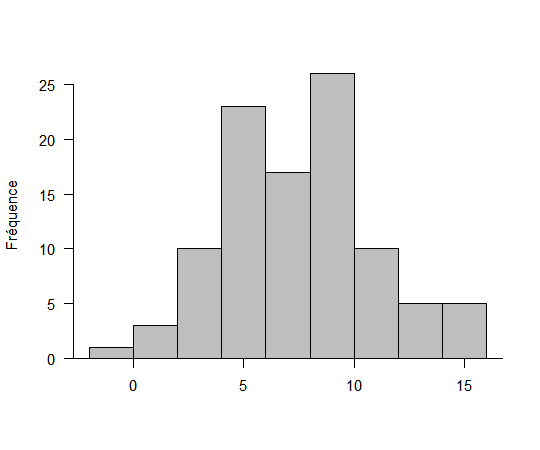
\includegraphics[width=3.5cm]{hist1.png}
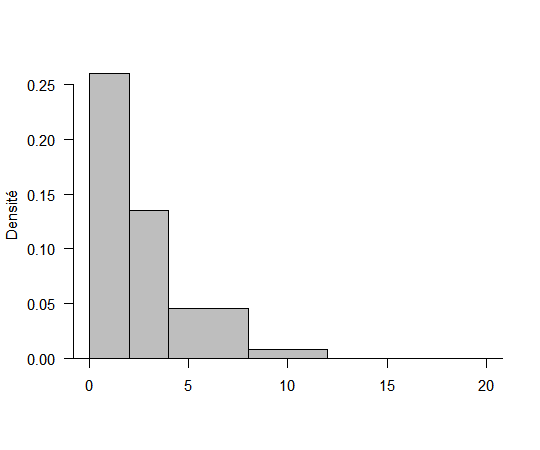
\includegraphics[width=3.5cm]{hist2.png}
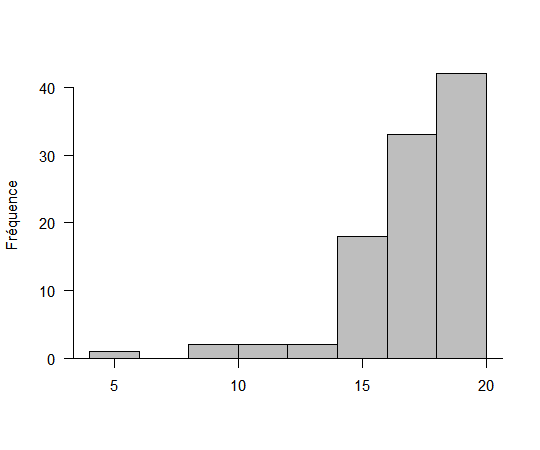
\includegraphics[width=3.5cm]{hist3.png}

\begin{itemize}
\item L'histogramme sert à \alerter{estimer une fonction de densité à partir d'un échantillon}.
\item Il aide à juger si un modèle probabiliste est approprié pour la population d'où provient l'échantillon.
\item Si l'histogramme est en forme de cloche (\alerter{unimodal} et \alerter{symétrique}), nous serons à
l'aise avec le postulat de normalité de la population.
\end{itemize}
\end{frame}


\begin{frame}[t]{Tracer un histogramme}

{\small
Soit un échantillon $x_1,\ldots,x_n$.
\begin{itemize}\itemsep1pt
\item<1-> On divise l'ensemble des valeurs possibles de $X$ en environ 5 à 10 classes (intervalles de même
largeur ou non).
\item<2-> Soit $K$, le nombre de classes. On construit le tableau de fréquences contenant
\begin{itemize}\itemsep0pt
     \item[$n_j$ :] la fréquence (absolue), soit le nombre d'observations qui tombent dans la classe $j$,
     \item[$f_j$ :] \alerter{$f_j=n_j/n$}, la fréquence relative de la classe $j$, pour $j=1, \ldots, K$.
\end{itemize}
\item<3-> \alerter{La surface d'un rectangle doit être proportionnelle à sa fréquence relative.} Si $\ell_j$ est
la largeur de la classe $j$, alors $\ell_j\cdot h_j = c\cdot f_j$, où $c$ est une constante.
\item<3-> Classes égales : hauteurs égales aux fréquences absolues ou relatives.
\item<3-> Classes inégales : histogramme de densité ($c=1$), où \alert{$h_j=f_j/\ell_j$}.
\end{itemize}
}
\end{frame}


\begin{frame}[t]{Hauteur des rectangles d'un histogramme}

\begin{center}
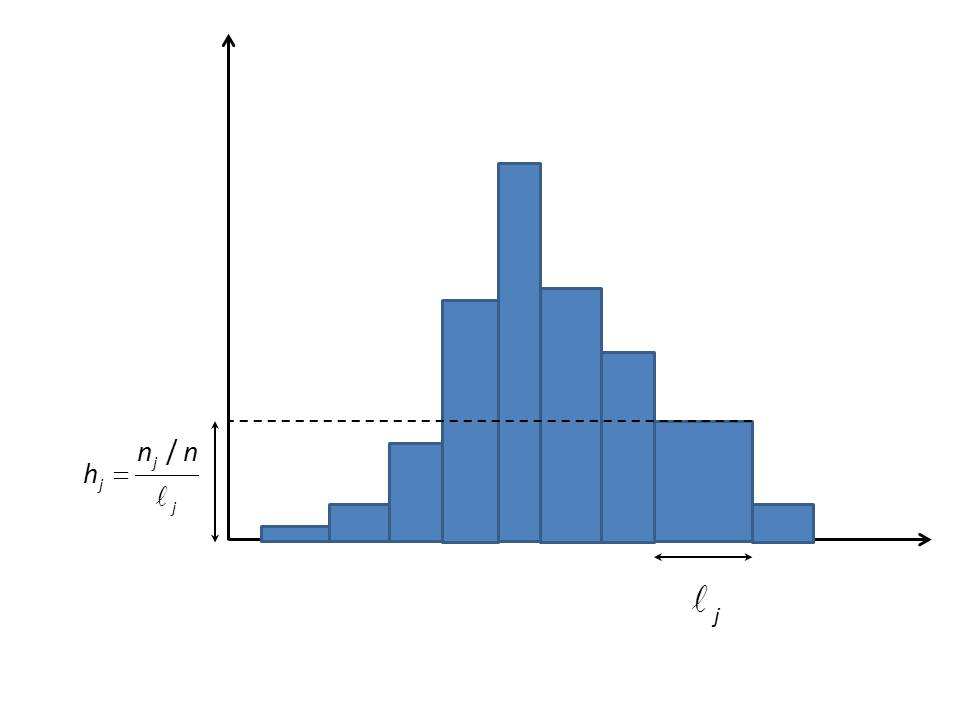
\includegraphics[height=6.6cm]{histog.jpg}
\end{center}
\end{frame}


\begin{frame}[t,label=exprocesseur]{Exemple 4 : utilisation du processeur}

{\small
On mesure à 50 moments le taux d'utilisation du processeur (en \%) d'un serveur peu sollicité.
On obtient les observations suivantes (en ordre croissant) :

\bigskip
\begin{tabular}{rrrrr rrrrr}
4,0 & 4,6 & 5,4 & 5,4  & 5,7  & 5,7  & 5,8  & 5,9  & 6,5  & 6,6 \\
6,6 & 6,7 & 6,8 & 6,8  & 7,0  & 7,0  & 7,1  & 7,1  & 7,2  & 7,3  \\
7,4 & 7,5 & 7,5 & 7,5  & 7,8  & 7,8  & 8,1  & 8,2  & 8,2  & 8,3  \\
8,7 & 8,8 & 8,8 & 8,9  & 8,9  & 9,1  & 9,3  & 9,4  & 9,5  & 9,6  \\
9,6 & 9,7 & 9,7 & 10,4 & 10,4 & 10,5 & 11,1 & 11,4 & 11,5 & 12,3\\
\end{tabular}

\bigskip
Tracez un histogramme dont les classes sont de largeur égale, et un autre dont les classes ont des largeurs
différentes.
}
\lienreponse{rep-ex}
\end{frame}


\begin{frame}[t]{Histogramme dont les classes sont de largeur égale}

Avec des classes de même largeur de la forme $(a, b]$ (la première inclut aussi sa borne inférieure),
l'histogramme a l'allure suivante, en fréquences relatives ou en fréquences absolues :

\medskip
\begin{center}
\begin{tikzpicture}
\begin{axis}[histo, name=g, width=6.0cm, height=5cm, xmin=3.6, xmax=13.4, ymax=0.21, xtick={4,6,...,12},
  ytick={0,0.05,...,0.2}, ylabel={Fréquence relative}]
  \addplot[ybar interval, fill=red!70, draw=black] coordinates
    {(4,0.04) (5,0.12) (6,0.16) (7,0.20) (8,0.18) (9,0.16) (10,0.06) (11,0.06) (12,0.02) (13,0)};
\end{axis}
\begin{axis}[histo, name=h, width=6.0cm, height=5cm, at={([xshift=1.0cm]g.outer east)}, anchor=outer west,
  xmin=3.6, xmax=14.4, ymax=20, xtick={4,6,...,14}, ytick={0,5,...,20}, ylabel={Fréquence absolue},
  yticklabel style={/pgf/number format/.cd, fixed, precision=0}]
  \addplot[ybar interval, fill=blue!65, draw=black] coordinates
    {(4,8) (6,18) (8,17) (10,6) (12,1) (14,0)};
\end{axis}
\end{tikzpicture}
\end{center}
\end{frame}


\begin{frame}[t]{Exemple 4 (suite)}

Complétez le tableau de fréquences qui définit 8 classes de valeurs.

\medskip
\begin{tabular}{ccccc}\hline
Classe ($j$) & Largeur ($\ell_j$) & Fréq. ($n_j$) & Fréq. rel. ($f_j$) & Hauteur ($h_j$) \\ \hline
$[4{,}0;\, 6{,}0]$ & \ \     &   & \ \     \  &  \ \   \  \\[2mm]
$(6{,}0;\, 7{,}0]$ & \  \    & 8 & \  \    \  &  \ \   \  \\[2mm]
$(7{,}0;\, 8{,}0]$ &  \ \   & 10 & \  \    \  &  \ \   \  \\[2mm]
$(8{,}0;\, 8{,}5]$ & \  0,5\ & 4 & \ \ 0,08 \  &  \ \  0,16 \  \\[2mm]
$(8{,}5;\, 9{,}0]$ & \ 0,5\  & 5 & \ \ 0,10  \  & \ \  0,20 \  \\[2mm]
$(9{,}0;\,10{,}0]$ & \  1\   & 8 & \  \ 0,16 \  & \ \  0,16 \  \\[2mm]
$(10{,}0;\,11{,}0]$ & \ 1 \  & 3 & \  \ 0,06 \  & \ \  0,06 \  \\[2mm]
$(11{,}0;\,13{,}0]$ & \ 2\   & 4 & \ \ 0,08  \  & \ \  0,04 \  \\ \hline
\end{tabular}
\lienreponse{rep-ex}
\end{frame}


\begin{frame}[t]{Histogramme avec classes de largeur inégale}

\begin{center}
\begin{tikzpicture}
\begin{axis}[histo, width=8cm, height=5.2cm, xmin=3.6, xmax=13.4, ymax=0.21, xtick={4,6,...,12},
  ytick={0,0.05,...,0.2}, ylabel={Densité}]
  \addplot[ybar interval, fill=green!45, draw=black] coordinates
    {(4,0.08) (6,0.16) (7,0.20) (8,0.16) (8.5,0.20) (9,0.16) (10,0.06) (11,0.04) (13,0)};
\end{axis}
\end{tikzpicture}
\end{center}

(Vous devriez être capable de produire un tel histogramme à la main à partir d'un échantillon.)

\end{frame}

% ----------------------------------------------------------------------------
\subsection{Diagramme en boîte (\textit{boxplot})}

\begin{frame}[t]{Diagramme en boîte}

{\small
Le \alerter{diagramme en boîte} (\textit{boxplot} ou diagramme de quartiles) permet aussi d'illustrer la
distribution d'une série d'observations.

Un diagramme en boîte a l'allure suivante :
}
\begin{center}
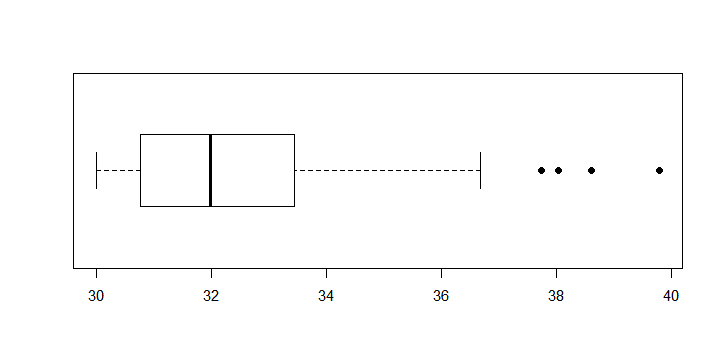
\includegraphics[width=8cm]{box-rien.png}
\end{center}
\end{frame}


\begin{frame}[t]{Construire un diagramme en boîte}

{\small
Un diagramme en boîte peut être tracé à la verticale ou à l'horizontale. Il est constitué
\begin{itemize}
\item<1-> d'un axe gradué;
\item<2-> d'une boîte dont les extrémités sont $Q_1=q_{0,25}$ et $Q_3=q_{0,75}$;
\item<2-> d'une ligne centrale au niveau de la médiane $Q_2$;
\item<3-> on calcule (\alerter{on ne trace PAS}) des bornes théoriques inférieure et supérieure :
\begin{align}
b_{inf}&=q_{0,25}-1,5\,EIQ\label{eq-binf}\\
b_{sup}&=q_{0,75}+1,5\,EIQ\label{eq-bsup}
\end{align}
\item<3-> d'un trait (« moustache ») de $Q_3$ jusqu'à \alerter{la plus grande valeur de l'échantillon
inférieure ou égale à $b_{sup}$};
\item<3-> d'un trait (« moustache ») de $Q_1$ jusqu'à \alerter{la plus petite valeur de l'échantillon
supérieure ou égale à $b_{inf}$};
\end{itemize}
}
\end{frame}


\begin{frame}[t,label=exbornes]{Construire un diagramme en boîte (suite)}

{\small
\begin{itemize}
\item<1-> de points pour chaque observation à l'extérieur de l'intervalle $[b_{inf},b_{sup}]$.
\end{itemize}
Les observations représentées par des points sur un diagramme en boîte sont parfois appelées
\textit{données aberrantes} ou \textit{données extrêmes}, puisqu'elles sont très peu plausibles sous une
loi normale.

\bigskip
\underline{Exercice} : remplacez les quartiles échantillonnaux par les quartiles théoriques d'une loi
$\mathcal{N}(\mu,\sigma^2)$ dans les équations (\ref{eq-binf}) et (\ref{eq-bsup}), et calculez
$P(X<b_{inf}\text{\ ou\ }X>b_{sup})$ si $X\sim \mathcal{N}(\mu,\sigma^2)$. Quelle est la probabilité
d'observer une valeur extrême, c'est-à-dire hors de $[b_{inf}, \, b_{sup}]$?
}
\lienreponse{rep-ex}
\end{frame}


\begin{frame}[t]{Utilité du diagramme en boîte}

{\small
Le diagramme en boîte permet d'évaluer en un coup d'œil certaines propriétés de la distribution des
observations :
\begin{itemize}
\item le centre de la distribution (mesuré par la médiane);
\item la dispersion (mesurée par l'écart interquartile);
\item la symétrie (l'écart entre le 1\textsuperscript{er} quartile et la médiane est-il le même que l'écart
entre la médiane et le 3\textsuperscript{e} quartile? les moustaches sont-elles de même longueur?);
\item la présence d'observations peu plausibles sous la loi normale (trop extrêmes).
\end{itemize}
}

Mais il est surtout idéal pour comparer plusieurs échantillons simultanément (voir diapo suivante).
\end{frame}


\begin{frame}[t]{Diagrammes en boîte juxtaposés}

\begin{center}
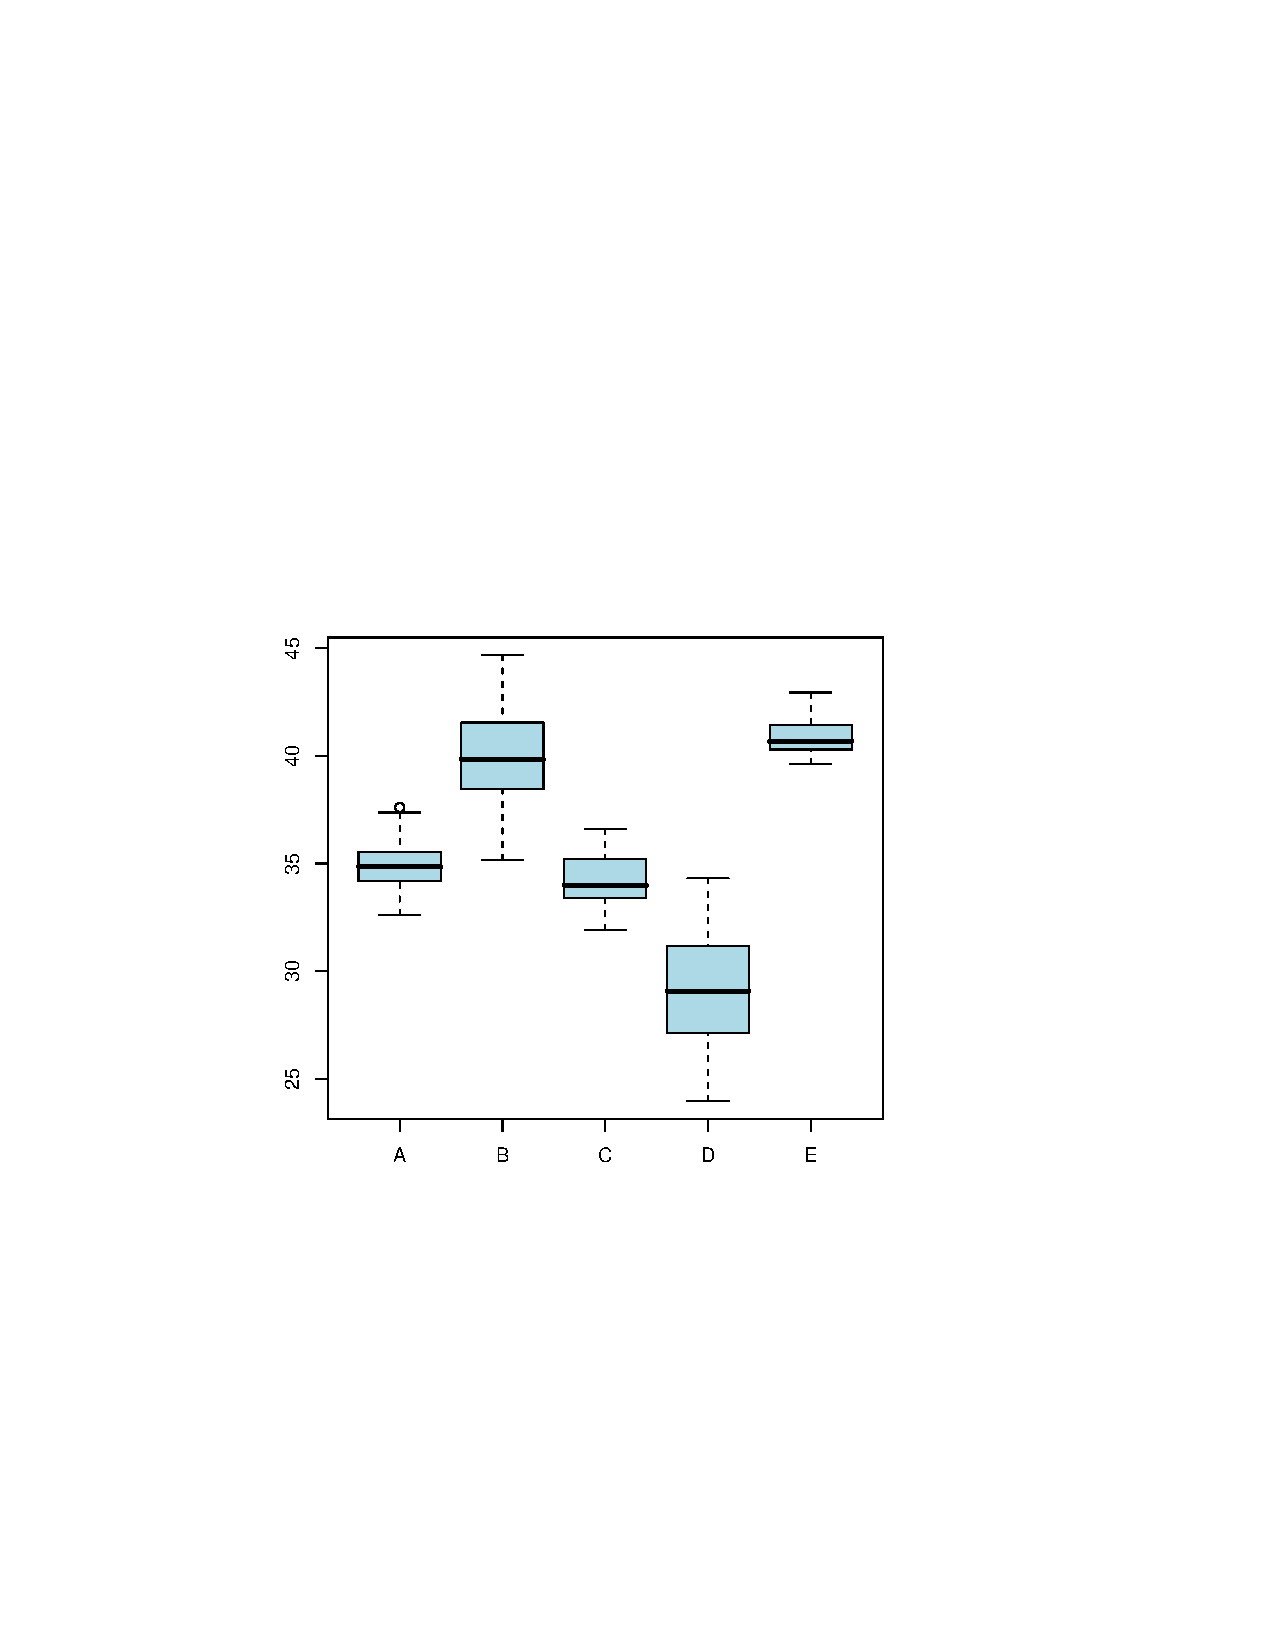
\includegraphics[width=8cm]{Diag_boite2.pdf}
\end{center}
\end{frame}


\begin{frame}[t,label=exboite]{Exercice (retour à l'exemple 4)}

Construisez à la main le diagramme en boîte des taux d'utilisation du processeur, et montrez qu'il a
l'allure suivante :

\begin{center}
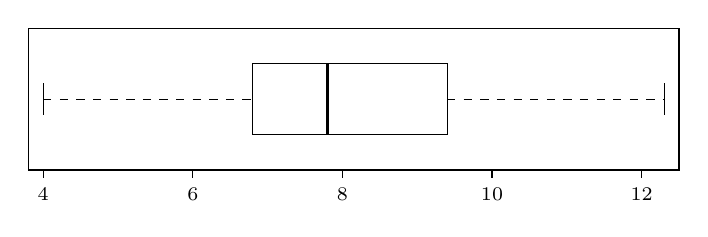
\begin{tikzpicture}[x=0.95cm]
  \draw (3.8,-0.9) rectangle (12.5,0.9);
  \foreach \t in {4,6,8,10,12} {
    \draw (\t,-0.9) -- (\t,-1.0) node[below] {\scriptsize \t};
  }
  \draw[dashed] (4.0,0) -- (6.8,0);
  \draw[dashed] (9.4,0) -- (12.3,0);
  \draw (4.0,-0.2) -- (4.0,0.2);
  \draw (12.3,-0.2) -- (12.3,0.2);
  \draw[fill=white] (6.8,-0.45) rectangle (9.4,0.45);
  \draw[very thick] (7.8,-0.45) -- (7.8,0.45);
\end{tikzpicture}
\end{center}
\lienreponse{rep-ex}
\end{frame}

% ============================================================================
\section{Réponses des exemples}

\begin{frame}[t,label=rep-ex]{Réponses des exemples}
\footnotesize
\begin{itemize}\itemsep3pt
\item \textbf{Exemple 1} (échantillon $8,17,2,11$) : $x_{(1)}=2$, $x_{(2)}=8$, $x_{(3)}=11$, $x_{(4)}=17$.
\item \retour{exquantiles}{Exemple 2 : quantiles} (échantillon ordonné $3,4,6,8,9$) :
$q_{0,3}=x_{(2)}=4$~; $q_{0,65}=x_{(3,75)}=6+0{,}75\times(8-6)=7{,}5$.
\item \retour{exquartiles}{Exemple 3 : quartiles} (échantillon ordonné $1,2,2,4,4,5,9,11,15,15,17$) :
$Q_1=x_{(3,25)}=2{,}5$, $Q_2=x_{(6)}=5$, $Q_3=x_{(8,75)}=14$, d'où $EIQ=11{,}5$~; $R=16$ et $s\approx5{,}9$.
\item \retour{exprocesseur}{Exemple 4 : utilisation du processeur} (tableau de fréquences) : $[4{,}0;6{,}0]$ :
$\ell_j=2$, $n_j=8$, $f_j=0{,}16$, $h_j=0{,}08$~; $(6{,}0;7{,}0]$ : $\ell_j=1$, $f_j=0{,}16$, $h_j=0{,}16$~;
$(7{,}0;8{,}0]$ : $\ell_j=1$, $f_j=0{,}20$, $h_j=0{,}20$.
\item \retour{exbornes}{Exercice : bornes sous la loi normale} : avec $Q_1=\mu-0{,}6745\sigma$,
$Q_3=\mu+0{,}6745\sigma$ et $EIQ\approx1{,}349\sigma$, on obtient $b_{inf}=\mu-2{,}70\sigma$ et
$b_{sup}=\mu+2{,}70\sigma$, d'où $P(X<b_{inf}\text{ ou }X>b_{sup})\approx 0{,}007$ (0,7\,\%).
\item \retour{exboite}{Exercice : diagramme en boîte} : $Q_1=x_{(13)}=6{,}8$, $Q_2=7{,}8$, $Q_3=x_{(38)}=9{,}4$,
$EIQ=2{,}6$, $b_{inf}=2{,}9$, $b_{sup}=13{,}3$~: aucune donnée extrême, les moustaches vont jusqu'au minimum
($4{,}0$) et au maximum ($12{,}3$) de l'échantillon.
\end{itemize}
\end{frame}

% ============================================================================
\section{Réponses des quiz}

\begin{frame}[t,label=rep-quiz]{Réponses des quiz}
\footnotesize
\begin{itemize}\itemsep3pt
\item \retour{quizmoy}{Quiz : moyenne} : faux, retirer le maximum et le minimum change généralement la
moyenne (sauf coïncidence).
\item \retour{quizmu}{Quiz : comparaison de $\mu$ et $\widetilde\mu$} : pour la loi uniforme (symétrique),
$\mu=\widetilde\mu=11$, comme pour toute loi symétrique~; pour la seconde loi (asymétrique à droite),
$\mu>\widetilde\mu$.
\item \retour{quizmed}{Quiz : médiane} : vrai, pour $n=30$ (pair), retirer le maximum et le minimum ne
change pas les deux valeurs centrales de l'échantillon ordonné, donc la médiane est inchangée.
\end{itemize}
\end{frame}


\begin{frame}{Bibliographie}
 	Ce document est rédigé avec Beamer ainsi qu'une classe .cls fournie par Jérôme Soucy. Les diapositives sont adaptées des diapositives créées par Thierry Duchesne et Emmanuelle Reny-Nolin pour le cours STT-1900.
 	\printbibliography
 	\vfill
 	\footnotesize Pour signaler une erreur dans ce document, veuillez écrire à l'adresse :~\href{mailto:julien.miron@mat.ulaval.ca}{julien.miron@mat.ulaval.ca}.
 \end{frame}

\end{document}
